\documentclass{article}

\usepackage{wrapfig}
\usepackage{amssymb}
\usepackage{polski}
\usepackage[polish]{babel}
\usepackage[utf8]{inputenc}
\usepackage[T1]{fontenc}
\usepackage{libertine}
\usepackage{graphicx}
\usepackage{multicol}
\usepackage{fancyhdr}
\usepackage[a4paper,headheight=65pt,bottom=65pt]{geometry}
\usepackage{lastpage}

\pagestyle{fancy}
\fancyhf{}
\fancyhead[L]{Podlaski Turniej w~Programowaniu Zespołowym 2015\\ Politechnika Białostocka, 21-22 marca 2015}
\fancyhead[R]{
\includegraphics[scale=0.7]{logoturnieju.png}}
\fancyfoot[L]{Problem B: Franki}
\fancyfoot[R]{\thepage/\pageref{LastPage}}
\renewcommand{\footrulewidth}{0.4pt}

\begin{document}
\begin{center}
  \begin{Huge}
    Problem B: Franki
  \end{Huge}
\end{center}

Aby zapobiec destrukcyjnemu oddziaływaniu rosnącej ceny franka szwajcarskiego na kondycję banków polskich, Zarząd
NBP wprowadził następującą ustawę o międzybankowym lokowaniu kapitału.

Dla każdej pary banków należy wynegocjować stopień ryzyka $SR_{ij}$ lokaty kapitału banku B i w inwestycje prowadzone
przez bank $B_{j}$. Takie negocjacje powinny być prowadzone ostatniego dnia każdego miesiąca a ustalany stopień ryzyka $SR_{ij}$
powinien zależeć od kondycji finansowych obu banków ($B_{i}$ oraz $B_{j}$) oraz dochodu banku $B_{i}$ uzyskanego z lokaty w inwestycje
banku $B_{j}$ w okresie ostatnich 30 / 31 dni.

Banki mogą inwestować jedynie w \textit{bezpieczne lokaty} i tylko w obrębie banków będących w \textit{relacji wzajemnego poręczenia}.

\section*{Pouczenie}

\textit{Bezpieczna lokata} -- lokata kapitału banku B i~w~inwestycje banku $B_{j}$ jest bezpieczna, jeśli wartość $m \cdot (1-SR_{ij})$ ($m$ jest
współczynnikiem bezpieczeństwa) jest większa od różnicy ceny franka i~ceny euro (tj. gdy $m \cdot (1-SR_{ij}) >$ CHF$ - $EUR$)$
($m\in N_{+}$, $SR_{ij}$ jest liczbą rzeczywistą z~przedziału (0,1)). Na rys.~bezpieczna lokata kapitału banku $B_{i}$~w~inwestycje banku $B_{j}$
jest oznaczana krawędzią zorientowaną <$i$,$j$>.

\begin{wrapfigure}{r}{0.3\textwidth}
  \begin{center}
    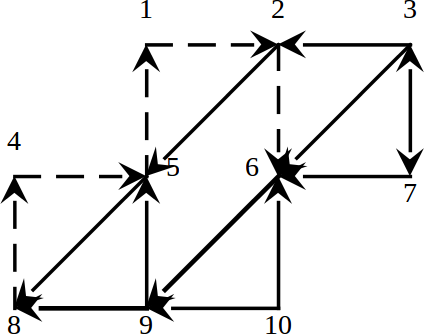
\includegraphics[width=2in]{B1.png}
  \end{center}
  \caption{Rysunek pierwszy}
  \label{fig:one}
\end{wrapfigure}

Bank $B_{i}$ \textit{może poręczyć} za inwestycje banku $B_{j}$, jeśli istnieje ścieżka bezpiecznych lokat
prowadząca z~banku $B_{i}$~do banku $B_{j}$. (patrz rys.~\ref{fig:one}:~Bank $B_{8}$ może poręczyć za inwestycje banku $B_{6}$, ponieważ istnieje ścieżka $8 \rightarrow 4 \rightarrow 5 \rightarrow 1 \rightarrow 2 \rightarrow 6$ bezpiecznych lokat prowadząca z~banku $B_{8}$ do banku $B_{6}$.)

Banki $B_{i}$~i~$B_{j}$ są w~relacji wzajemnego poręczenia, jeśli bank $B_{i}$ może poręczyć za inwestycje banku $B_{j}$ i~na odwrót (patrz rys.~Banki $B_{6}$ i~$B_{8}$ są w~relacji wzajemnego poręczenia, ponieważ istnieją ścieżki bezpiecznych lokat w~obie strony, tj. $6 \rightarrow 9 \rightarrow 8$ i~$8 \rightarrow 4 \rightarrow 5 \rightarrow 1 \rightarrow 2 \rightarrow 6$).

\section*{Wejście}
W~pierwszej linii wejścia podane są następujące wartości oddzielone pojedynczą spacją: $n$ - liczba banków ($1 < n < 10^4$),
$m$ -- współczynnik bezpieczeństwa ($1 < m < 10^4$), \textit{CHF} -- cena franka, \textit{EUR} -- cena euro ($1 \le $EUR$, $CHF$ \le 10^4$), $k$ -- numer
banku $B_{k}$, $t$ -- numer banku $B_{t}$ ($1 < k, t \leqslant n$).

W~kolejnych $n$ liniach podana jest macierz \textit{SR} (o~rozmiarze $n \times n$) zawierająca liczby zmiennoprzecinkowe (z~przedziału ($0$,$1$))
reprezentujące stopnie ryzyka między wszystkimi parami banków, tzn. wartość \textit{SR}[i][j] macierzy oznacza stopień ryzyka
lokaty kapitału banku $B_{i}$~w~inwestycje prowadzone przez bank $B_{j}$. Zakładamy, że banki są numerowane od~$1$.

\section*{Wyjście}

W~pierwszej linii wyjścia należy wypisać (oddzielając pojedynczą spacją) numery wszystkich banków, które są w~relacji
wzajemnego poręczenia z~bankiem $B_{k}$.

W~drugiej linii należy wypisać (oddzielając pojedynczą spacją) numery wszystkich banków, które są w~relacji
wzajemnego poręczenia z~bankiem $B_{t}$.
Ciąg numerów banków w~obu przypadkach powinien być uporządkowany rosnąco.
Jeśli banki $B_{k}$ i~$B_{t}$ są w~relacji wzajemnego poręczenia, obie linie powinny być identyczne.

\newpage
\section*{Przykład}
dane wejściowe:
\begin{verbatim}
10 5 8.26 6.01 1 3
0.95 0.14 0.84 0.71 0.84 0.95 0.97 0.63 0.74 0.88
0.85 0.95 0.96 0.63 0.13 0.34 0.85 0.73 0.84 0.95
0.83 0.36 0.64 0.66 0.56 0.26 0.16 0.88 0.97 0.87
0.71 0.64 0.86 0.89 0.26 0.88 0.86 0.88 0.97 0.98
0.23 0.84 0.86 0.89 0.76 0.86 0.87 0.17 0.98 0.87
0.96 0.74 0.76 0.86 0.87 0.67 0.76 0.68 0.38 0.76
0.85 0.63 0.46 0.76 0.87 0.27 0.76 0.87 0.99 0.97
0.85 0.73 0.87 0.35 0.67 0.76 0.66 0.87 0.79 0.76
0.74 0.84 0.64 0.56 0.17 0.65 0.86 0.29 0.66 0.87
0.74 0.94 0.64 0.86 0.76 0.18 0.65 0.86 0.15 0.67
\end{verbatim}
\begin{wrapfigure}{r}{0.5\textwidth}
  \begin{center}
    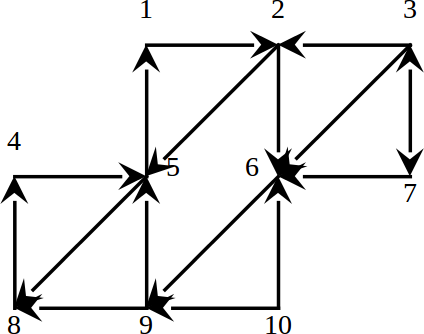
\includegraphics[width=2in]{B2.png}
  \end{center}
  \caption{Rysunek dla danych wejściowych}
  \label{fig:two}
\end{wrapfigure}
wynik:
\begin{verbatim}
1 2 4 5 6 8 9
3 7
\end{verbatim}
\end{document}
